\documentclass[subsection=false]{beamer}
\setbeamertemplate{footline}[frame number] % numerar slides
\setbeamertemplate{navigation symbols}{} % retirar barra de navega��o

\mode<presentation>
\usetheme{Singapore}

\ifdefined\hyperref  

\usepackage[brazil]{babel}
\usepackage[latin1]{inputenc}
\usepackage{graphicx}
\usepackage{subcaption}  
\usepackage{pgfpages}
\usepackage{ifpdf}   
\usepackage{multimedia}  
\usepackage{color}   
\usepackage{url} 
\usepackage{hyperref}
\usepackage{lastpage}

\pgfdeclareimage[width=0.85cm, height=1.10cm]{ufpa}{Figures/logo_ufpa}
\logo{\pgfuseimage{ufpa}}

\hypersetup{
	pdftitle={ASR e TTS Embarcado para Controle de TV}
	pdfauthor={Cassio Trindade Batista}
}
\fi

\title[ASR + TTS: Controle de Equipamentos Eletr�nicos\hspace{2.10cm}\thepage/\pageref{LastPage}]
{\Large Uso de Reconhecedor e Sintetizador de Voz Embarcados para
Controle de Equipamentos Eletr�nicos via Luz Infravermelha}
%{Uso de Reconhecedor e Sintetizador de Voz para Controle de Equipamentos Eletr�nicos}

\author[Cassio, Pedro, Gabriel e Thiago]{
\small
Cassio Trindade Batista\\
Gabriel Peixoto de Carvalho\\
Pedro Henrique C. F. Soares\\
Thiago Barros Coelho}

\institute{
\scriptsize
Universidade Federal do Par�\\
Instituto de Tecnologia\\
Faculdade de Engenharia da Computa��o e Telecomunica��es\\
Disciplina: Projetos de Hardware e Interfaceamento\\
Professores: Jeferson Leite e Adalbery Castro\\
\begin{figure}
	
\includegraphics[width=.11\textwidth]{Figures/logo_ufpa}
\end{figure}
\vspace{-.6cm}
}
\date{\small{25 de junho de 2015}}

\begin{document}
\begin{frame}[plain]
	\titlepage
\end{frame}

\section{Introdu��o}
\subsection{Introdu��o}
\begin{frame}{Introdu��o}
\begin{itemize}
	\item 23\% dos brasileiros possuem necessidades especiais
	\item Teclado e Mouse: Exclus�o digital
	\item Acessibilidade: Novas formas de controle
\end{itemize}
\begin{figure}
	
\includegraphics[width=.7\textwidth]{Figures/accessibility}
\end{figure}
\end{frame}

\section{Objetivos}
\subsection{Objetivos}
\begin{frame}{Objetivos}
\begin{itemize}
	\item Controlar uma TV por um smartphone Android atrav�s da voz
	\item Servidor de voz instalado na BeagleBone Black
	\item Microfone no cliente Android
	\item Transmissor de Sinais Infravermelhos configurado no Arduino
	\item Servidor LAMP para armazenamento de comandos configurado na BBB
\end{itemize}
\end{frame}

\begin{frame}{Esquem�tico do Projeto}
\begin{figure}
	\includegraphics[width=\textwidth]{Figures/schematic}
\end{figure}
\end{frame}

\begin{frame}{Cliente Android}
\begin{figure}
	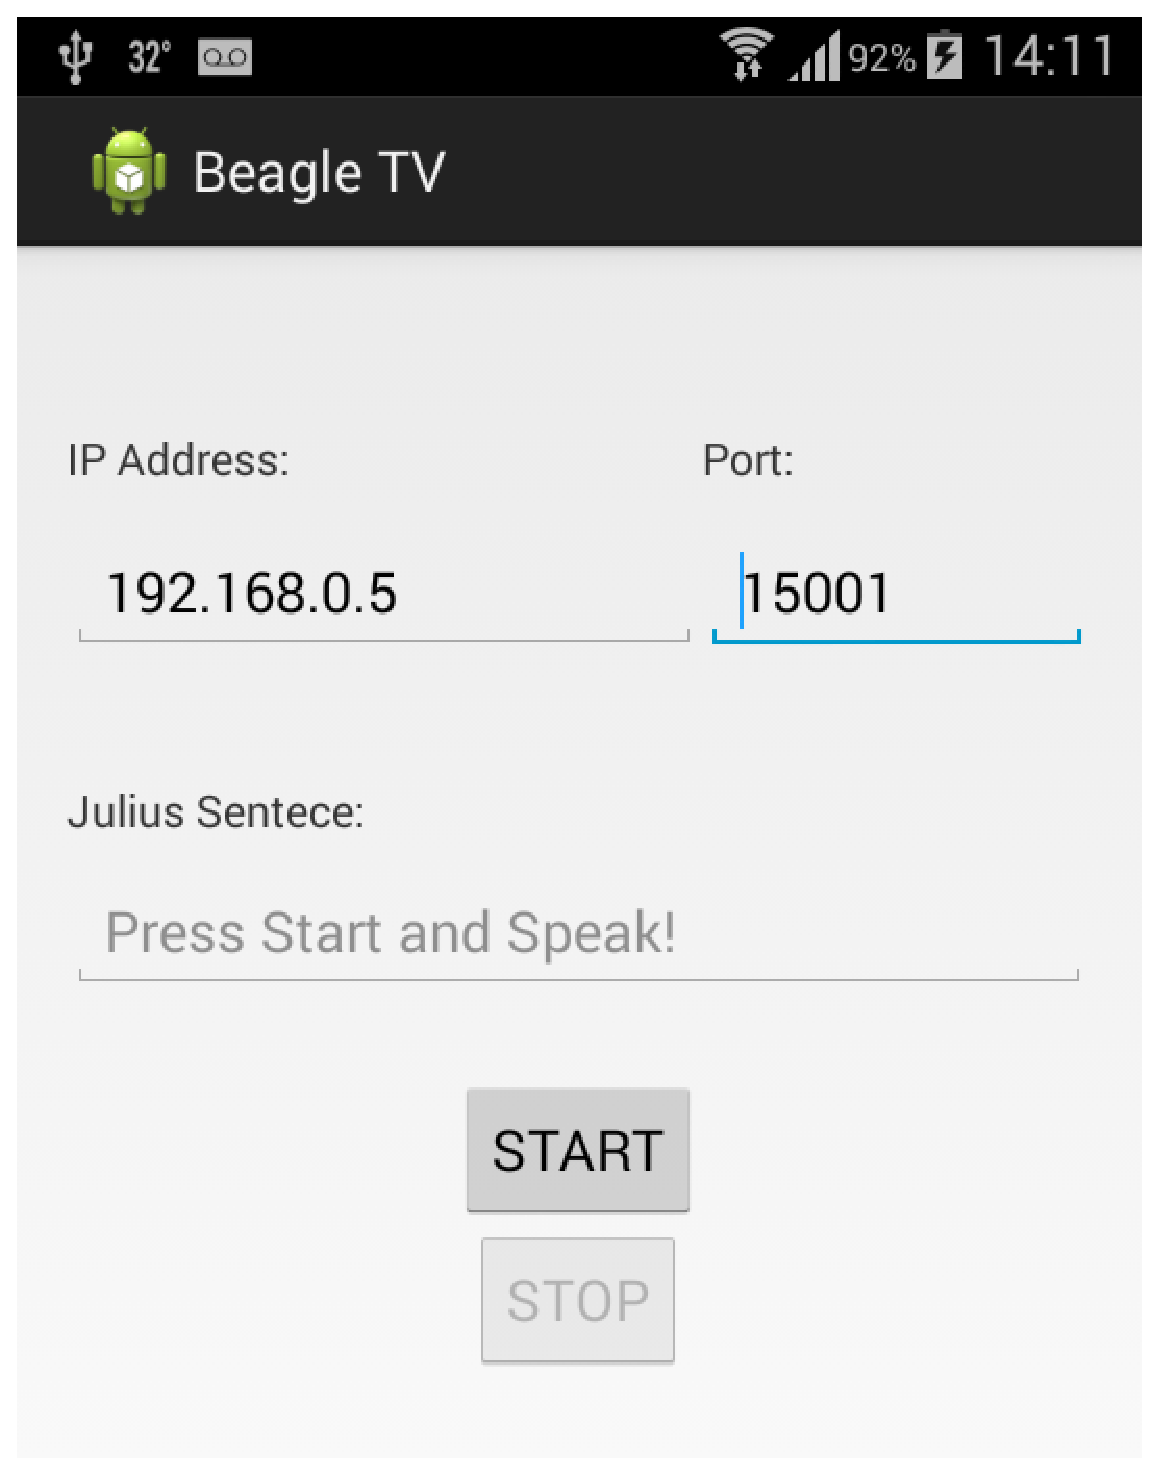
\includegraphics[width=.5\textwidth]{Figures/app}
\end{figure}
\end{frame}

\section{Teoria}
\subsection{Teoria}
\begin{frame}{Reconhecimento \textit{vs.} S�ntese}
\begin{figure}
	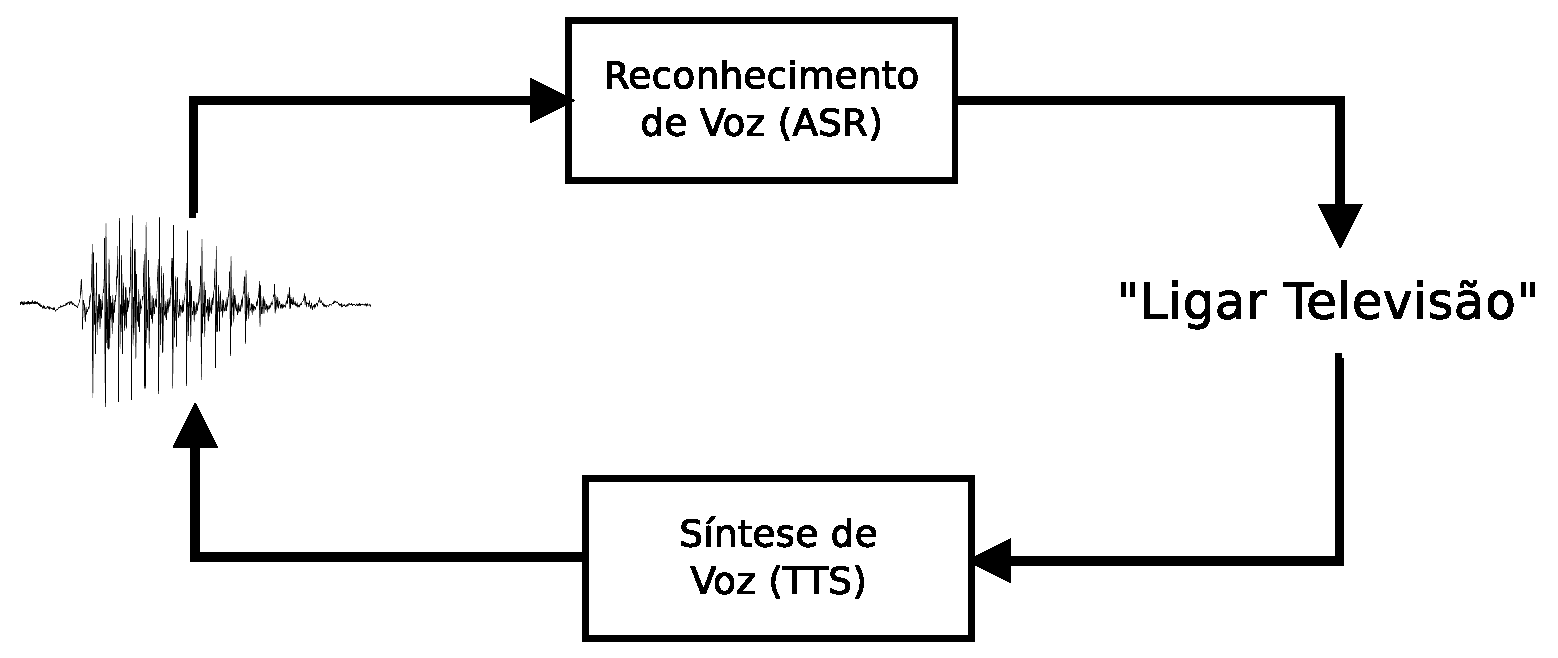
\includegraphics[width=\textwidth]{Figures/asr_tts}
\end{figure}
\end{frame}

\begin{frame}{Reconhecimento \textit{vs.} S�ntese}
\begin{figure}
	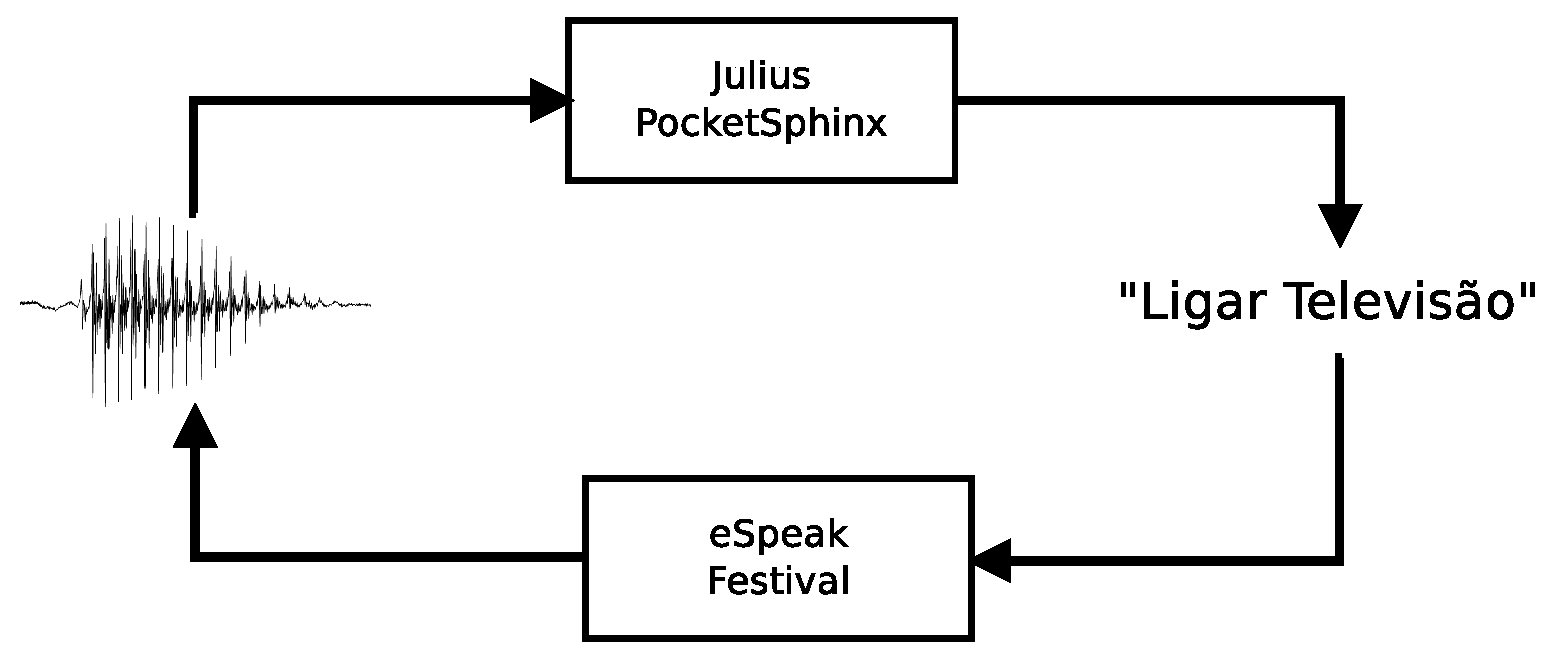
\includegraphics[width=\textwidth]{Figures/asr_tts_soft}
\end{figure}
\end{frame}

\begin{frame}{ASR: Reconhecimento Autom�tico de Voz}
\begin{figure}
	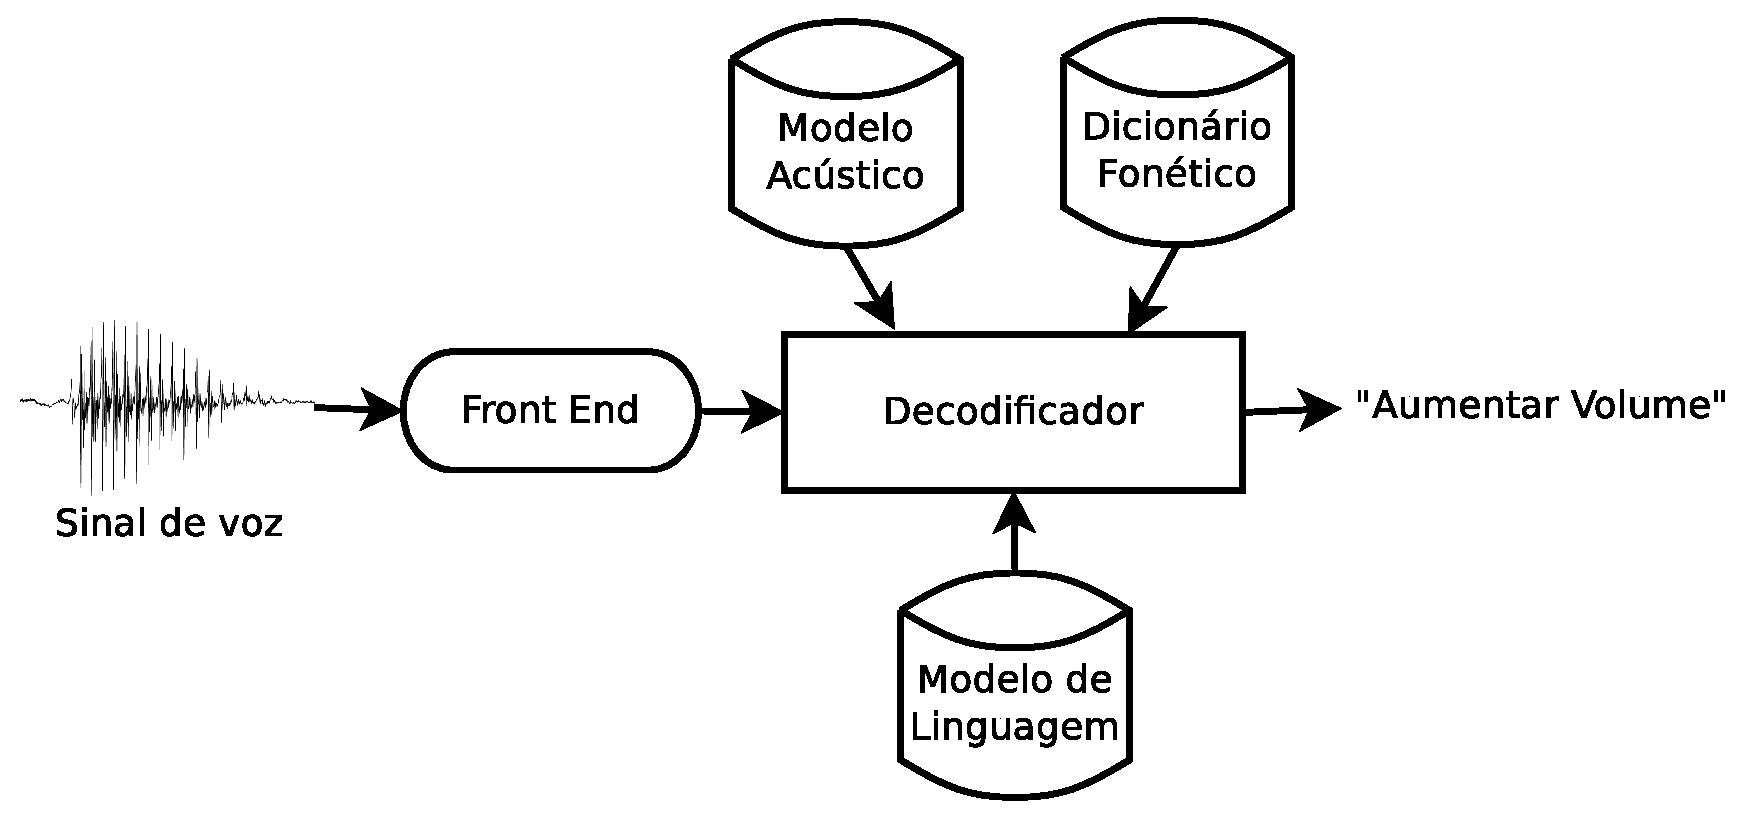
\includegraphics[width=\textwidth]{Figures/asr_sch}
\end{figure}
\end{frame}

\begin{frame}{PWM: Modula��o por Largura de Pulso}
\begin{figure}
	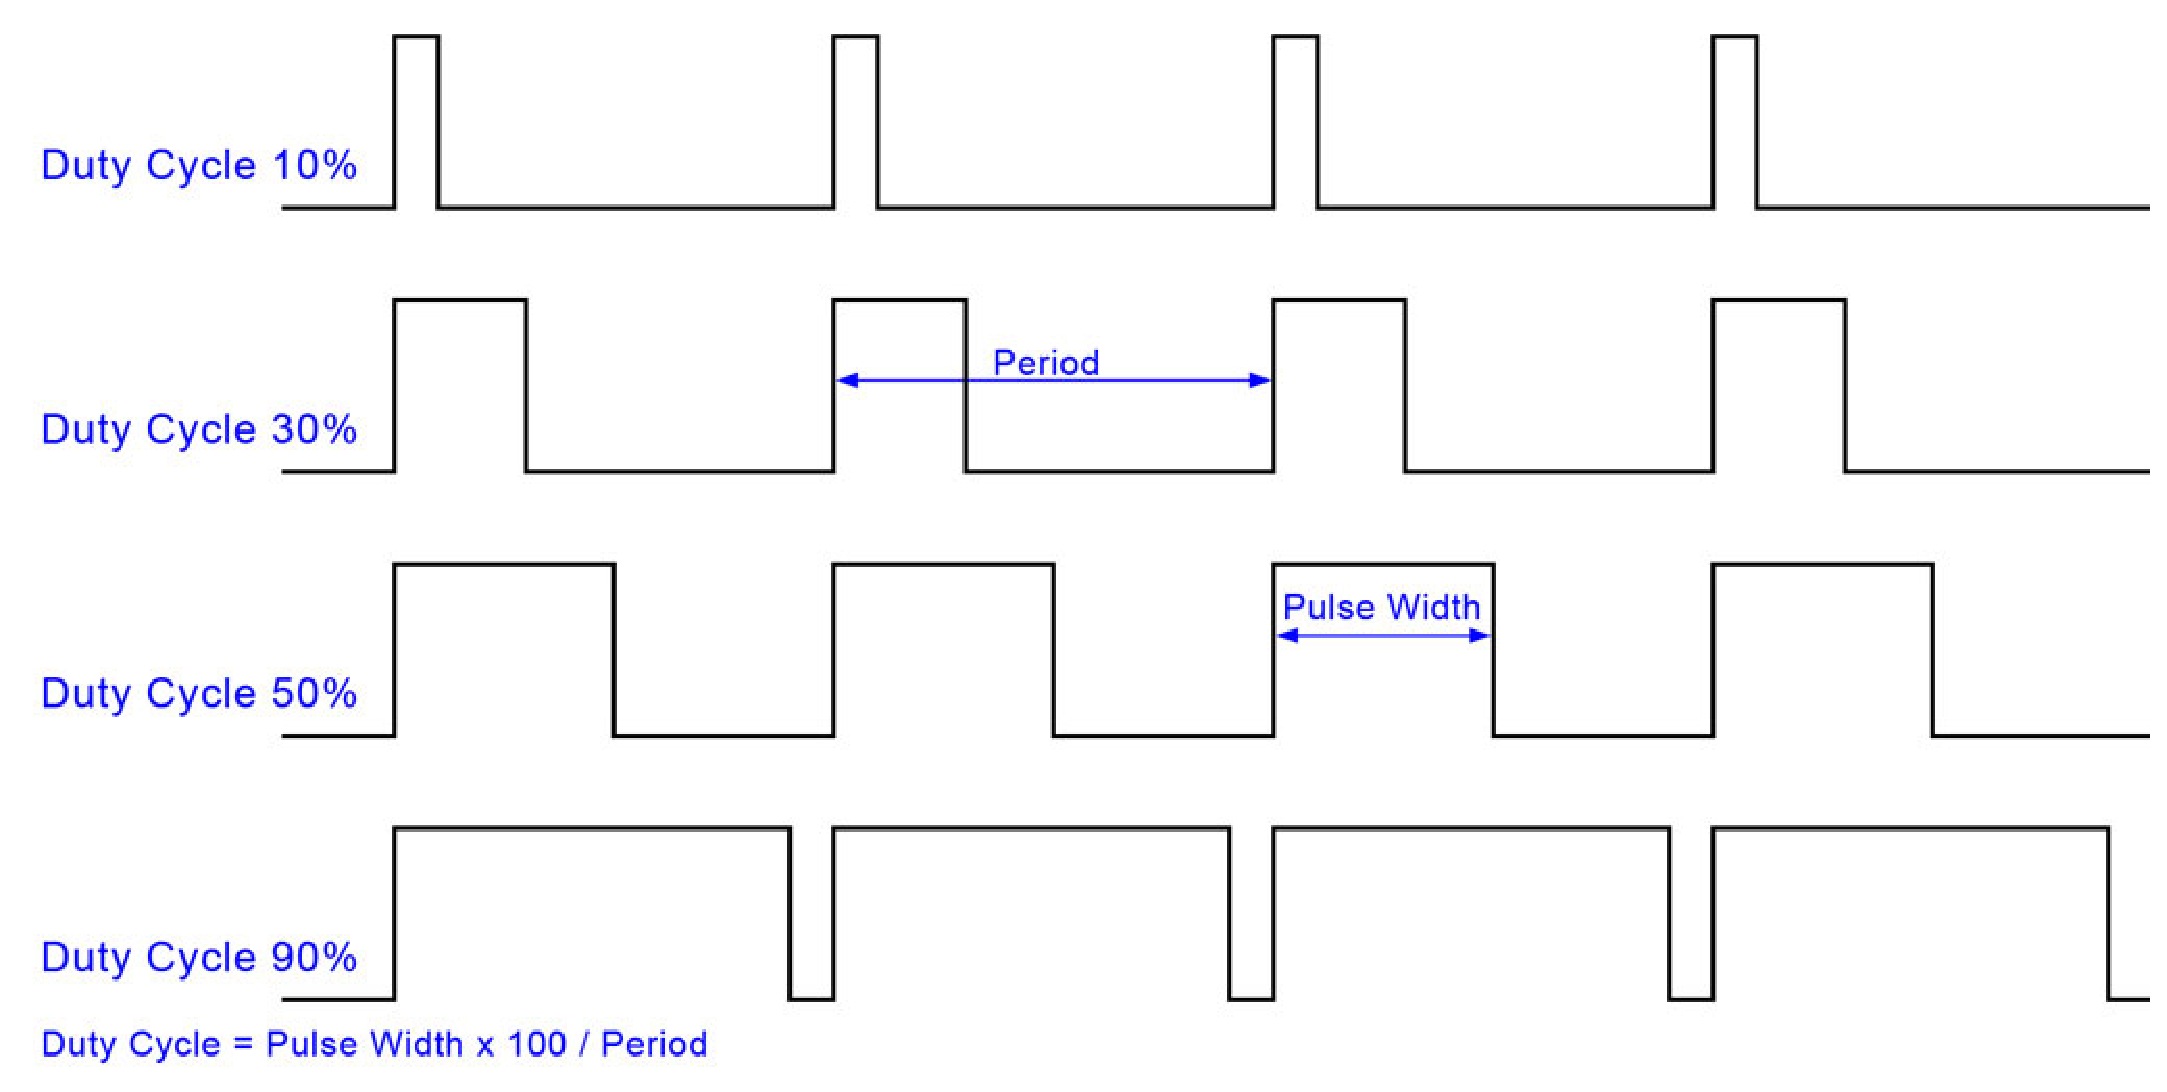
\includegraphics[width=.95\textwidth]{Figures/pwm}
\end{figure}
\end{frame}

\section{Protocolo IR}
\subsection{Protocolo IR}
\begin{frame}{Protocolo Philips RC-5}
\begin{figure}
	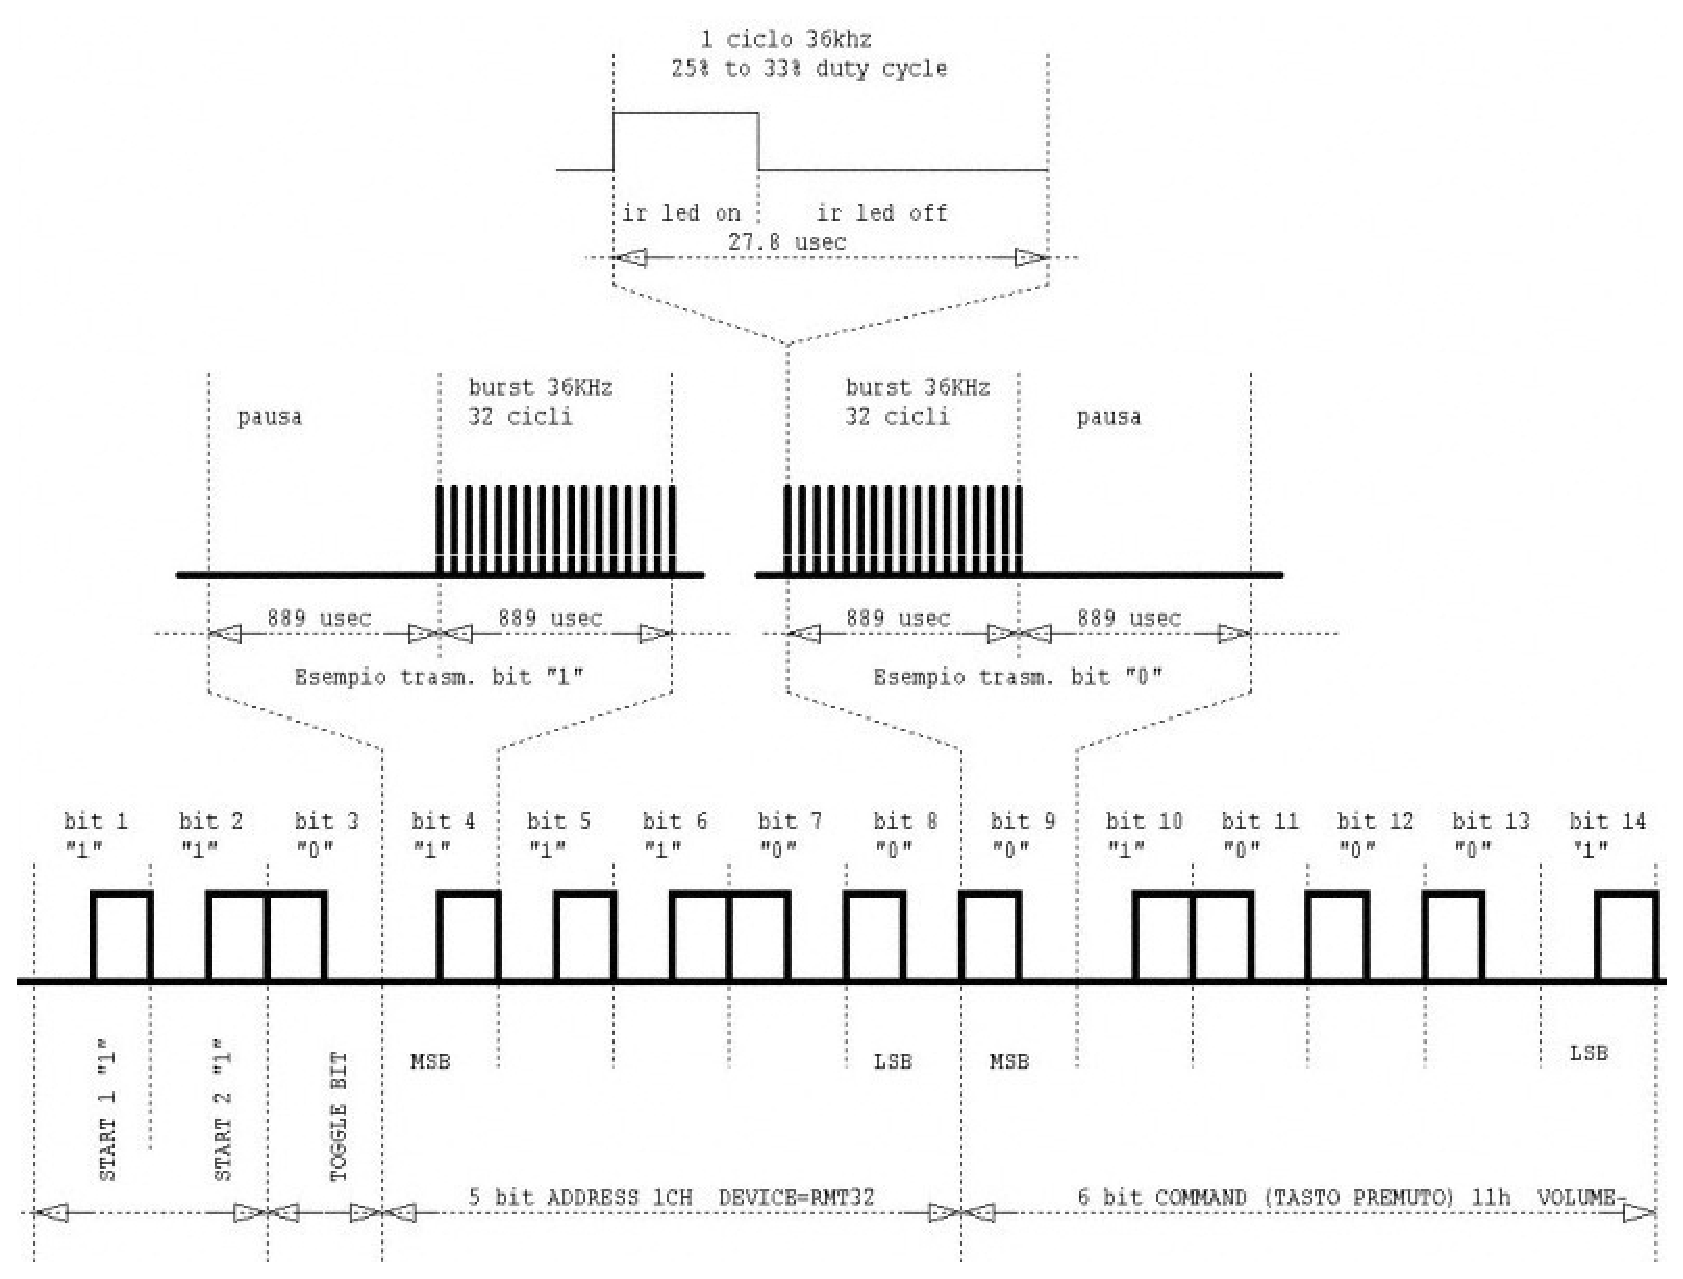
\includegraphics[width=.9\textwidth]{Figures/sch_rc5}
\end{figure}
\end{frame}

\begin{frame}{Protocolo Philips RC-6 (Plot)}
\begin{figure}
	\includegraphics[width=\textwidth]{Figures/cmds}
\end{figure}
\end{frame}

\begin{frame}{Protocolo Samsung}
\begin{figure}
	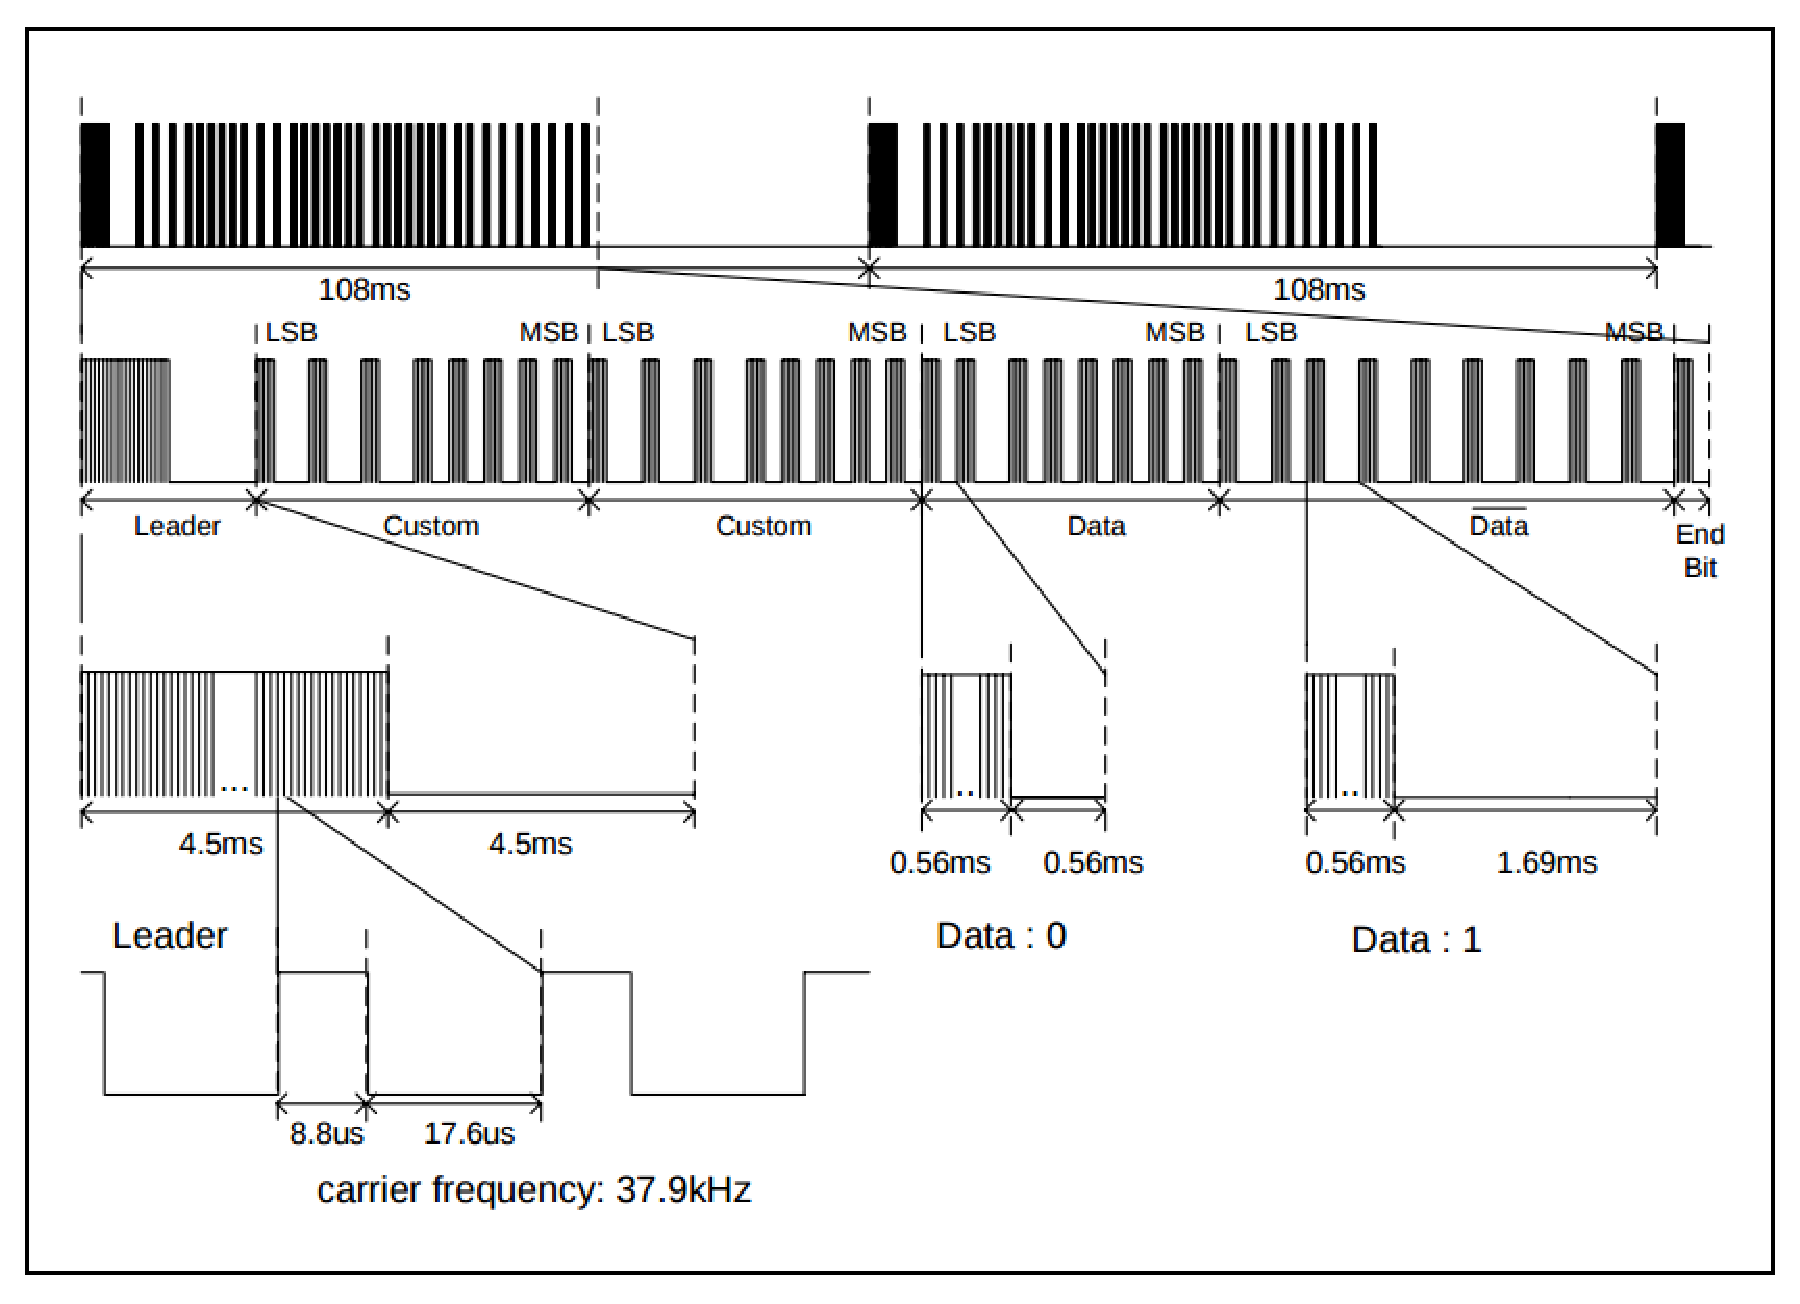
\includegraphics[width=.9\textwidth]{Figures/samsung_protocol}
\end{figure}
\end{frame}

\begin{frame}{Protocolo Samsung (Plot)}
\begin{figure}
	\includegraphics[width=\textwidth]{Figures/cmds_samsung}
\end{figure}
\end{frame}

\section{Tx/Rx}
\subsection{Tx/Rx}
\begin{frame}{Comunica��o BeagleBone $\rightarrow$ Arduino}
\begin{figure}
	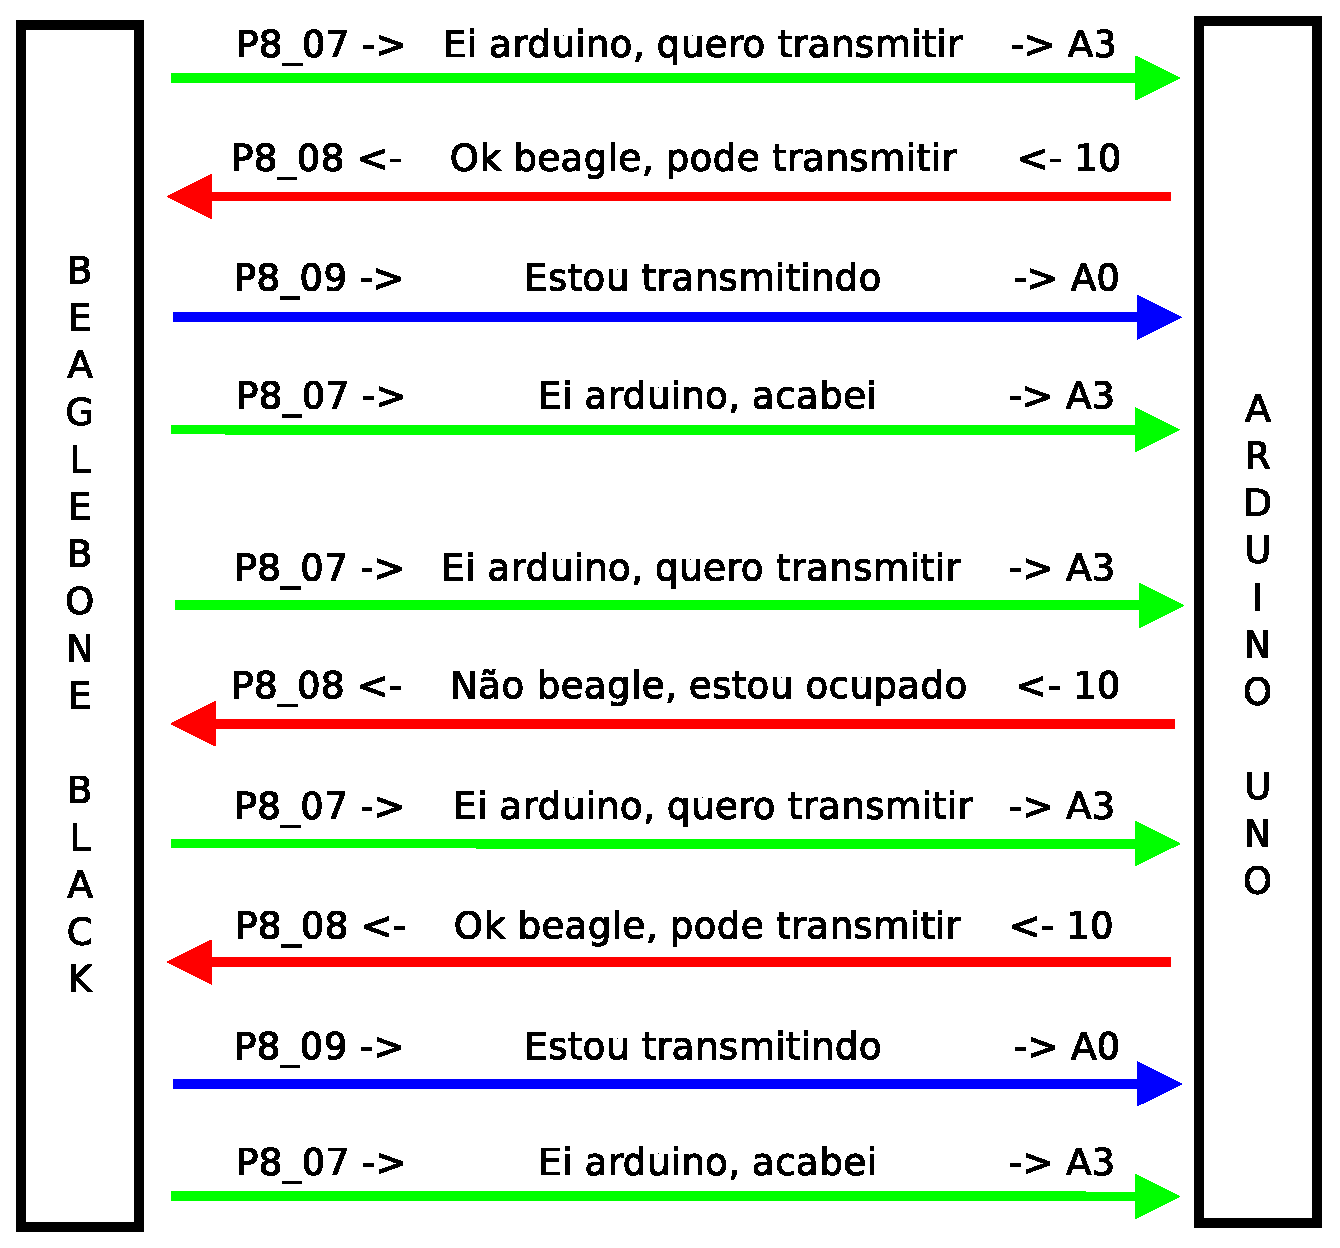
\includegraphics[width=.65\textwidth]{Figures/duplex_tx}
\end{figure}
\end{frame}

\section{VLW!}
\begin{frame}{Obrigado!}
\centering
\Huge
Perguntas?
\begin{figure}
	
\includegraphics[width=.30\textwidth]{Figures/question}
\end{figure}
\end{frame}
\end{document}
%%% EOF %%%
